\documentclass[10pt, a4paper]{article}

\usepackage{ctex}
\usepackage{xeCJK}
\usepackage{caption}
\usepackage{geometry}
\geometry{
    left = 0.6in,
    right = 0.6in,
    top = 0.8in,
    bottom = 1.0in
}
\usepackage{amssymb}
\usepackage{amsbsy}
\usepackage{amsmath}
\usepackage{xcolor}
\usepackage{mathrsfs}
\usepackage{graphicx}
\usepackage{pifont}
\usepackage{tasks}
\settasks{
    label = \Alph*. ,
    label-width = 16pt
}
\pagestyle{empty}

\newcommand{\Title}[3]{
    \begin{center}
        \Large \textbf{中国电子学会 #1~年~#2~月 Scratch~#3级考试}
    \end{center}
}
\newcommand{\TimeAndName}[1]{
    \begin{center}
        考试时间:~#1~ 分钟 \qquad\qquad\qquad\qquad 姓名:\underline{\quad\quad\quad\quad}
    \end{center}
}

\begin{document}
    \Title{2022}{9}{二} % 标题
    \TimeAndName{60} % 考试时间及姓名

    % 单选题
    \vspace{2mm}
    {\noindent\textbf{第一部分、单选题(共 25 题,每题 2 分,共50分.)}}
    \begin{enumerate}
        % 1
        \item 数列:1,2,3,4,6,9,13,19,28,...的下一项是多少?(\qquad)
        \begin{tasks}(4)
            \task 37
            \task 39
            \task 41
            \task 47
        \end{tasks}

        % 2
        \item 下图红框中填入下列哪个选项,能让角色在移动过程中碰到鼠标指针说“你挡着我了!”?(\qquad)
        \begin{tasks}(4)
            \task 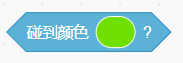
\includegraphics[width=.16\textwidth]{2a.png}
            \task 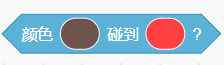
\includegraphics[width=.18\textwidth]{2b.png}
            \task 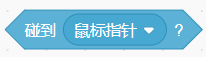
\includegraphics[width=.18\textwidth]{2c.png}
            \task 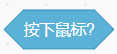
\includegraphics[width=.12\textwidth]{2d.png}
        \end{tasks}

        \begin{figure}[htbp]
            \centering
            \begin{minipage}[t]{.2\textwidth}
                \centering
                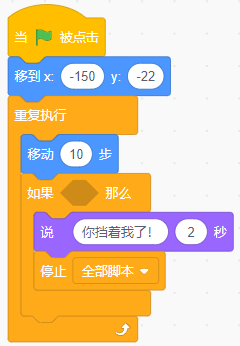
\includegraphics[width=\textwidth]{2.png}
                \caption*{第 2 题}
            \end{minipage}
            \begin{minipage}[t]{.26\textwidth}
                \centering
                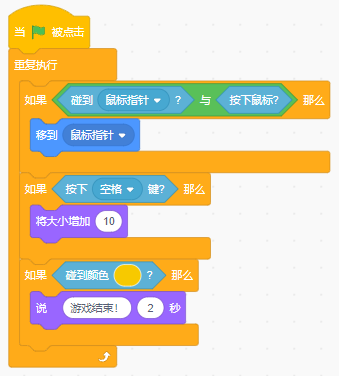
\includegraphics[width=\textwidth]{3.png}
                \caption*{第 3 题}
            \end{minipage}
            \begin{minipage}[t]{.24\textwidth}
                \centering
                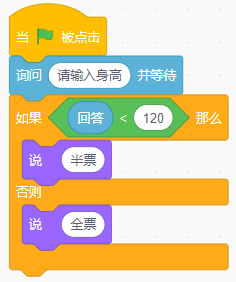
\includegraphics[width=\textwidth]{6.png}
                \caption*{第 6 题}
            \end{minipage}
        \end{figure}

        % 3
        \item 运行上图程序,说法正确的是?(\qquad)
        \begin{tasks}
            \task 在任何地方点击鼠标,角色都会移动到鼠标位置
            \task 当按下空格键后,执行角色大小增加10,当角色充满屏幕时,大小不再增加
            \task 在没有任何操作的时候,角色会在舞台区乱走
            \task 当碰到红色,说“游戏结束”2 秒,程序停止运行
        \end{tasks}

        % 4
        \item 小明想写一个程序实现如果用键盘输入的数字小于60就改变角色的特效,否则就使角色大小增加60,应该选择下列哪个积木?(\qquad)
        \begin{tasks}(4)
            \task 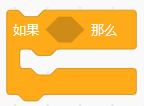
\includegraphics[width=.15\textwidth]{4a.png}
            \task 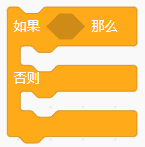
\includegraphics[width=.11\textwidth]{4b.png}
            \task 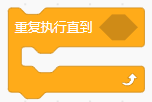
\includegraphics[width=.15\textwidth]{4c.png}
            \task 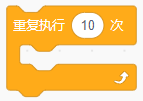
\includegraphics[width=.15\textwidth]{4d.png}
        \end{tasks}

        % 5
        \item 下列数学运算中,结果为60的是?(\qquad)
        \begin{tasks}(4)
            \task 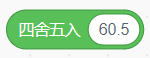
\includegraphics[width=.12\textwidth]{5a.png}
            \task 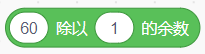
\includegraphics[width=.17\textwidth]{5b.png}
            \task 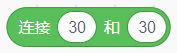
\includegraphics[width=.15\textwidth]{5c.png}
            \task 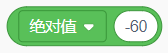
\includegraphics[width=.15\textwidth]{5d.png}
        \end{tasks}

        % 6
        \item 运行如上图程序,输入120,正确的显示效果是?(\qquad)
        \begin{tasks}(4)
            \task 全票
            \task 半票
            \task 半票全票
            \task 全票半票
        \end{tasks}

        \newpage
        % 7
        \item 如图所示,想让角色向右移动100步,应该采用哪个程序实现?(\qquad)
        \begin{tasks}(4)
            \task 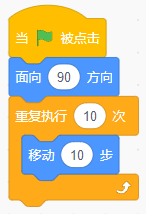
\includegraphics[width=.1\textwidth]{7a.png}
            \task 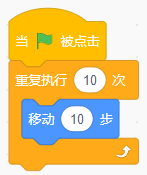
\includegraphics[width=.12\textwidth]{7b.png}
            \task 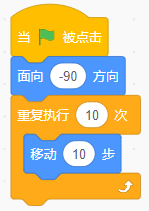
\includegraphics[width=.1\textwidth]{7c.png}
            \task 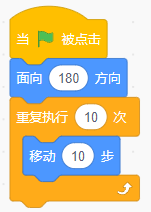
\includegraphics[width=.1\textwidth]{7d.png}
        \end{tasks}

        % 8
        \item Beetle初始方向如下左图所示,执行下右图程序后,Bettle的方向与下面哪个选项执行后相同?(\qquad)
        \begin{tasks}(4)
            \task 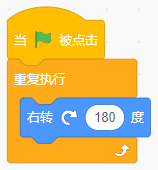
\includegraphics[width=.13\textwidth]{8a.png}
            \task 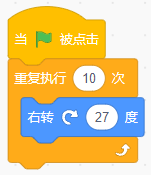
\includegraphics[width=.12\textwidth]{8b.png}
            \task 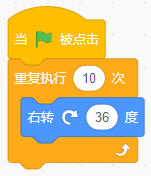
\includegraphics[width=.12\textwidth]{8c.png}
            \task 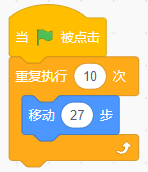
\includegraphics[width=.12\textwidth]{8d.png}
        \end{tasks}

        \begin{figure}[htbp]
            \centering
            \begin{minipage}[t]{.18\textwidth}
                \centering
                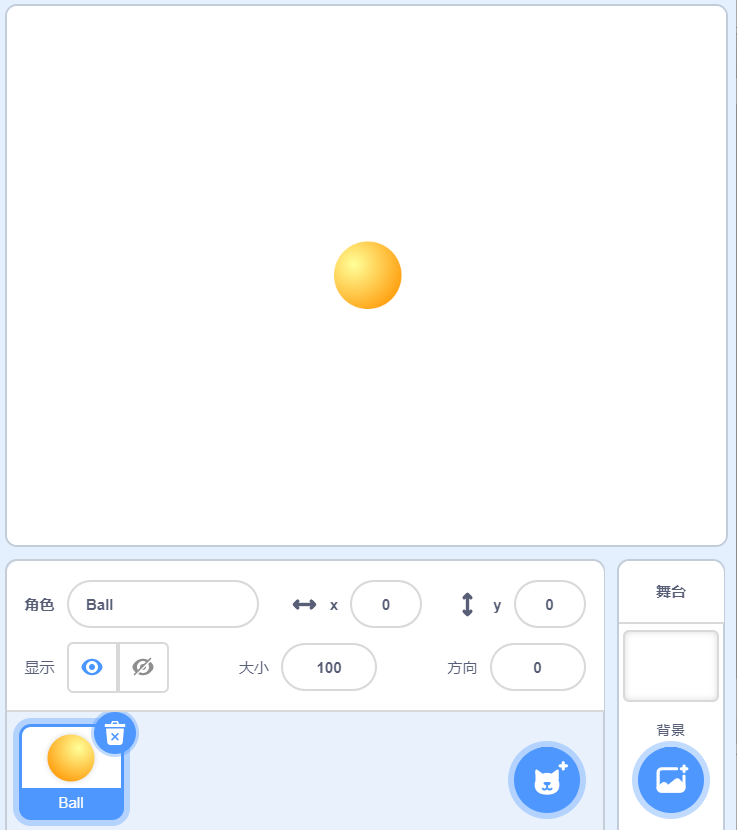
\includegraphics[width=\textwidth]{7.png}
                \caption*{第 7 题}
            \end{minipage}
            \begin{minipage}[t]{.4\textwidth}
                \centering
                \begin{minipage}[t]{.4\textwidth}
                    \centering
                    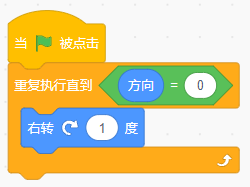
\includegraphics[width=\textwidth]{8-1.png}
                \end{minipage}
                \begin{minipage}[t]{.5\textwidth}
                    \centering
                    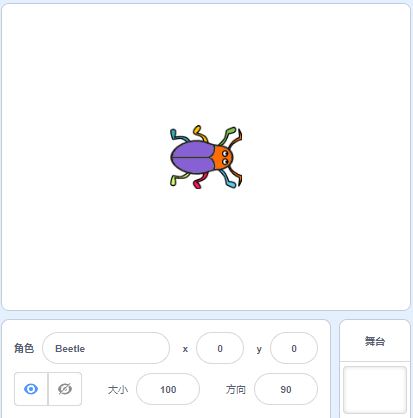
\includegraphics[width=\textwidth]{8-2.png}
                \end{minipage}
                \caption*{第 8 题}
            \end{minipage}
            \begin{minipage}[t]{.28\textwidth}
                \centering
                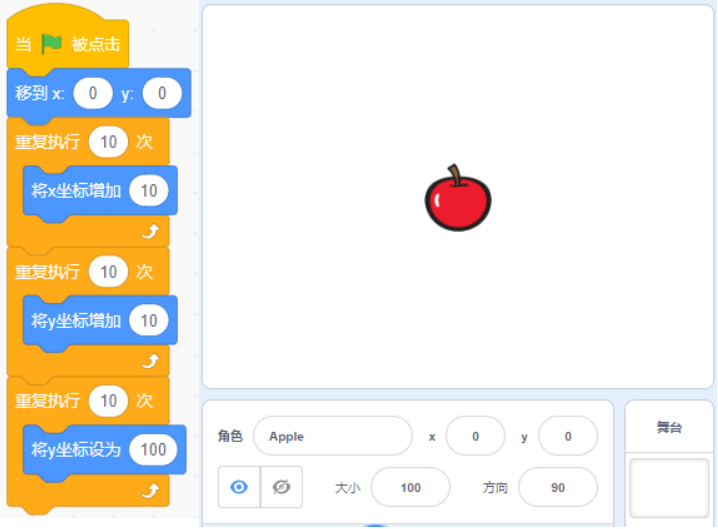
\includegraphics[width=\textwidth]{9.png}
                \caption*{第 9 题}
            \end{minipage}
            \begin{minipage}[t]{.12\textwidth}
                \centering
                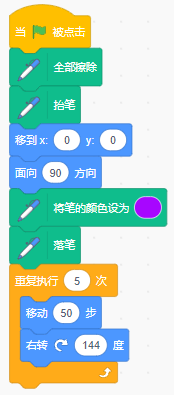
\includegraphics[width=\textwidth]{12.png}
                \caption*{第 12 题}
            \end{minipage}
        \end{figure}

        % 9
        \item 运行上图程序,角色的最终坐标为?(\qquad)
        \begin{tasks}(4)
            \task $(100,-100)$
            \task $(100,100)$
            \task $(-100,100)$
            \task $(100,0)$
        \end{tasks}

        % 10
        \item 运行下列程序,说法正确的是?(\qquad)
        
        \begin{minipage}{.6\textwidth}
            \begin{tasks}
                \task 程序会一直重复执行下去,任何情况下都不会停止
                \task 角色在移动过程中一直切换造型
                \task 角色会一直移动到按下鼠标,然后停下来,并换成下一个造型
                \task 角色会一直移动到按下鼠标,然后停下来,不切换造型
            \end{tasks}
        \end{minipage}
        \begin{minipage}{.3\textwidth}
            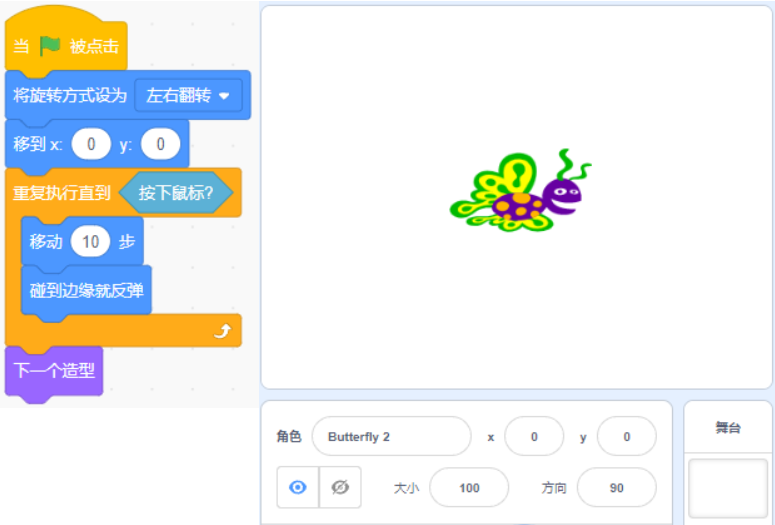
\includegraphics[width=\textwidth]{10.png}
        \end{minipage}
        
        % 11
        \item 角色初始状态如图所示,运行下列程序,说法正确的是?(\qquad)
        
        \begin{minipage}{.3\textwidth}
            \centering
            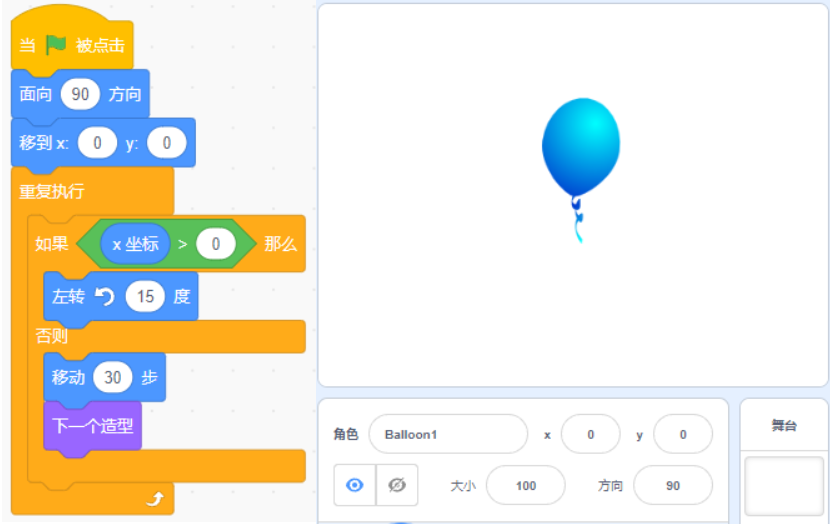
\includegraphics[width=\textwidth]{11.png}
        \end{minipage}
        \begin{minipage}{.63\textwidth}
            \begin{tasks}
                \task 程序开始运行,角色立即旋转
                \task 程序开始运行,角色向右移动30步并切换造型,然后开始不停旋转
                \task 程序开始运行,角色向右移动30步,开始旋转
                \task 程序开始运行,角色向右移动30步并切换造型,左转15度后静止不动
            \end{tasks}
        \end{minipage}

        % 12
        \item 运行上图程序,画出的图形是?(\qquad)
        \begin{tasks}(4)
            \task 五边形
            \task 六边形
            \task 正方形
            \task 五角星
        \end{tasks}

        \newpage
        % 13
        \item 下列哪个选项结果为true?(\qquad)
        \begin{tasks}(4)
            \task 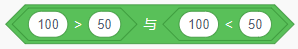
\includegraphics[width=.18\textwidth]{13a.png}
            \task 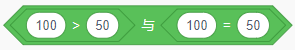
\includegraphics[width=.18\textwidth]{13b.png}
            \task 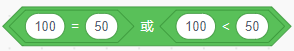
\includegraphics[width=.18\textwidth]{13c.png}
            \task 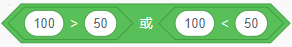
\includegraphics[width=.18\textwidth]{13d.png}
        \end{tasks}

        % 14
        \item 田径场上正在进行100米决赛,参加决赛的是A、B、C、D、E、F六个人,关于谁会得冠军,看台上甲、乙、丙谈了自己的看法。甲认为D、F都不可能是冠军;乙认为冠军不是A就是B;丙坚信冠军绝不是C。比赛结束后,人们发现他们三人中只有一个人的看法是正确的,请问谁是100米赛冠军?(\qquad)
        \begin{tasks}(4)
            \task A
            \task B
            \task C
            \task E
        \end{tasks}

        % 15
        \item 观察规律,红色空格内内应填入哪个选项?(\qquad)
        
        \begin{minipage}{.2\textwidth}
            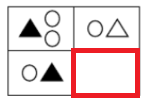
\includegraphics[width=.5\textwidth]{15.png}
        \end{minipage}
        \begin{minipage}{.7\textwidth}
            \begin{tasks}(4)
                \task 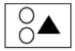
\includegraphics[width=.12\textwidth]{15a.png}
                \task 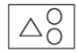
\includegraphics[width=.12\textwidth]{15b.png}
                \task 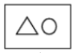
\includegraphics[width=.12\textwidth]{15c.png}
                \task 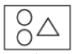
\includegraphics[width=.12\textwidth]{15d.png}
            \end{tasks}
        \end{minipage}

        % 16
        \item 下列哪个按钮,可以让整段声音变小一点儿?(\qquad)
        \begin{tasks}(4)
            \task 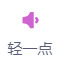
\includegraphics[width=.06\textwidth]{16a.png}
            \task 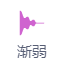
\includegraphics[width=.06\textwidth]{16b.png}
            \task 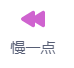
\includegraphics[width=.06\textwidth]{16c.png}
            \task 
\includegraphics[width=.06\textwidth]{16d.png}
        \end{tasks}

        % 17
        \item 积木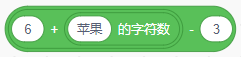
\includegraphics[width=.2\textwidth]{17.png}的运行结果是?(\qquad)
        \begin{tasks}(4)
            \task 5
            \task 3
            \task 6
            \task 8
        \end{tasks}

        \begin{figure}[htbp]
            \centering
            \begin{minipage}[t]{.4\textwidth}
                \centering
                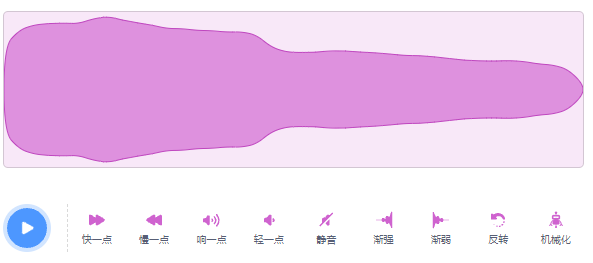
\includegraphics[width=\textwidth]{16.png}
                \caption*{第 16 题}
            \end{minipage}
            \begin{minipage}[t]{.22\textwidth}
                \centering
                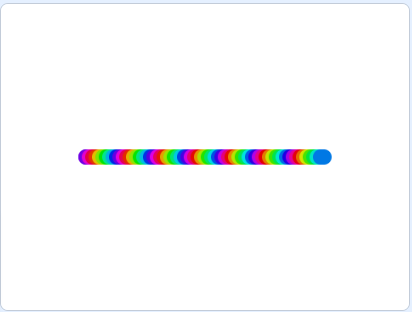
\includegraphics[width=\textwidth]{19.png}
                \caption*{第 19 题}
            \end{minipage}
            \begin{minipage}[t]{.22\textwidth}
                \centering
                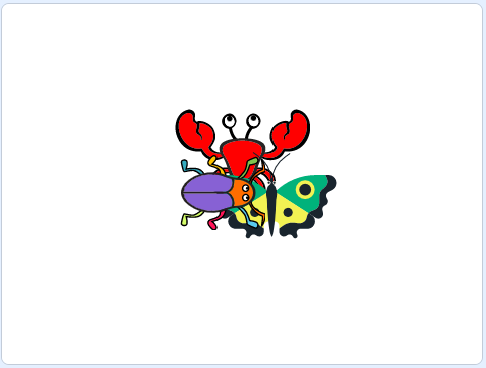
\includegraphics[width=\textwidth]{20.png}
                \caption*{第 20 题}
            \end{minipage}
            \begin{minipage}[t]{.09\textwidth}
                \centering
                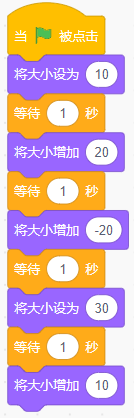
\includegraphics[width=\textwidth]{21.png}
                \caption*{第 21 题}
            \end{minipage}
        \end{figure}

        % 18
        \item 积木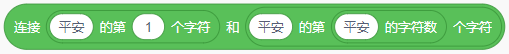
\includegraphics[width=.4\textwidth]{18.png}运行结果是?(\qquad)
        \begin{tasks}(4)
            \task 平安平安
            \task 平安
            \task 安平
            \task 安平安平
        \end{tasks}

        % 19
        \item 实现上图所示渐变色的效果,可以使用画笔里的哪个指令?(\qquad)
        \begin{tasks}(4)
            \task 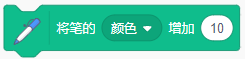
\includegraphics[width=.18\textwidth]{19a.png}
            \task \includegraphics[width=.18\textwidth]{19b.png}
            \task \includegraphics[width=.15\textwidth]{19c.png}
            \task \includegraphics[width=.15\textwidth]{19d.png}
        \end{tasks}

        % 20
        \item 三个角色的位置如上图所示,它们的层关系“从后到前”依次是?(\qquad)
        \begin{tasks}(4)
            \task 昆虫\ 蝴蝶\ 螃蟹
            \task 螃蟹\ 蝴蝶\ 昆虫
            \task 蝴蝶\ 螃蟹\ 昆虫
            \task 蝴蝶\ 昆虫\ 螃蟹
        \end{tasks}

        % 21
        \item 运行上图程序后,角色的大小是?(\qquad)
        \begin{tasks}(4)
            \task 50
            \task 30
            \task 20
            \task 40
        \end{tasks}

        \newpage
        % 22
        \item 	A、B、C、D四个队举行足球循环赛(即每两个队都要赛一场),胜一场得3分,平一场得1分,负一场得0分。 已知: 
        
        \ding{172}~比赛结束后四个队的得分都是奇数; 

        \ding{173}~A队总分第一; 

        \ding{174}~B队恰有两场平局,并且其中一场是与C队平局。 
        
        问:D队得几分?(\qquad)
        \begin{tasks}(4)
            \task 3
            \task 5
            \task 7
            \task 1
        \end{tasks}

        % 23
        \item 小丑鱼、螃蟹、海星身体上的橙色一样,下列选项是鲨鱼程序的一部分,下面哪个选项可以让鲨鱼碰到小丑鱼后说“吃掉小丑鱼了!”,碰到其他角色什么都不说?(\qquad)
        \begin{tasks}(4)
            \task \includegraphics[width=.18\textwidth]{23a.png}
            \task \includegraphics[width=.18\textwidth]{23b.png}
            \task \includegraphics[width=.18\textwidth]{23c.png}
            \task \includegraphics[width=.18\textwidth]{23d.png}
        \end{tasks}

        \begin{figure}[htbp]
            \centering
            \begin{minipage}[t]{.25\textwidth}
                \centering
                \includegraphics[width=\textwidth]{23.png}
                \caption*{第 23 题}
            \end{minipage}
            \begin{minipage}[t]{.4\textwidth}
                \centering
                \includegraphics[width=\textwidth]{24.png}
                \caption*{第 24 题}
            \end{minipage}
            \begin{minipage}[t]{.3\textwidth}
                \includegraphics[width=\textwidth]{25.png}
                \caption*{第 25 题}
            \end{minipage}
        \end{figure}

        % 24
        \item 角色在舞台的位置如图所示,运行下列程序,说法正确的是?(\qquad)
        \begin{tasks}
            \task 角色向右移动10步并切换造型
            \task 按下空格键,角色向右移动10步并切换造型
            \task 按下空格键以外的键,角色向右移动10步并切换造型
            \task 按下空格键,角色向左移动10步并切换造型
        \end{tasks}

        % 25
        \item 下列选项说法错误的是?(\qquad)
        \begin{tasks}(2)
            \task 舞台背景总是位于最下层
            \task 画笔画出的图案和图章位于同一层
            \task 从角色库中新添加的角色会自动出现在最上层
            \task 画笔画出的线条有时可以遮挡住其他角色
        \end{tasks}
    \end{enumerate}

    \newpage
    % 判断题
    {\noindent\textbf{第二部分、判断题(共 10 题,每题 2 分,共20分.)}}
    \begin{enumerate}
        \setcounter{enumi}{25}
        % 26
        \item 程序中要判断角色是否碰到舞台边缘,可以使用运动模块中的“碰到舞台边缘”积木. (\qquad)

        % 27
        \item 运行下列程序,每次按下空格键,角色大小都会增加10. (\qquad)

        % 28
        \item 下列两个程序的运行结果一样. (\qquad)

        % 29
        \item 点击绿旗,运行下列程序,草莓最后的大小为110. (\qquad)

        \begin{figure}[htbp]
            \centering
            \begin{minipage}[t]{.4\textwidth}
                \centering
                \includegraphics[width=\textwidth]{28.png}
                \caption*{第 28 题}
            \end{minipage}
            \begin{minipage}[t]{.43\textwidth}
                \centering
                \includegraphics[width=\textwidth]{29.png}
                \caption*{第 29 题}
            \end{minipage}
            \begin{minipage}[t]{.15\textwidth}
                \centering
                \includegraphics[width=\textwidth]{30.png}
                \caption*{第 30 题}
            \end{minipage}
        \end{figure}

        % 30
        \item 运行上图程序,按下鼠标键,角色会在舞台上一直运动并切换造型. (\qquad)

        % 31
        \item 角色初始方向和程序如图所示,运行程序后,角色回到初始方向. (\qquad)
        
        \begin{figure}[htbp]
            \centering
            \begin{minipage}[t]{.28\textwidth}
                \centering
                \includegraphics[width=\textwidth]{31.png}
                \caption*{第 31 题}
            \end{minipage}
            \begin{minipage}[t]{.18\textwidth}
                \centering
                \includegraphics[width=\textwidth]{34.png}
                \caption*{第 34 题}
            \end{minipage}
            \begin{minipage}[t]{.5\textwidth}
                \centering
                \begin{minipage}[t]{.4\textwidth}
                    \centering
                    \includegraphics[width=\textwidth]{35-1.png}
                \end{minipage}
                \begin{minipage}[t]{.5\textwidth}
                    \centering
                    \includegraphics[width=\textwidth]{35-2.png}
                \end{minipage}
                \caption*{第 35 题}
            \end{minipage}
        \end{figure}

        % 32
        \item 使用画笔模块中的“落笔”积木,可以在舞台上印出一个与角色相同的图案. (\qquad)

        % 33
        \item 数列:15, 8, 12, 8, 9, 8, ( ), ( ), ...,第一个空填6,第二个空填8. (\qquad)
        
        % 34
        \item 运行上图程序音量会增加10. (\qquad)

        % 35
        \item 角色的初始位置如上右图所示,运行如上左图所示的程序,角色在1秒内滑行到坐标$(100,-100)$. (\qquad)
    \end{enumerate}

    \newpage
    {\noindent \textbf{第三部分、编程题(共 2 题,共30分.)}}
    \begin{enumerate}
        \setcounter{enumi}{35}
        
        % 36
        \item 绘制图形:
        
        1. 准备工作
        \begin{tasks}[label = (\arabic*)]
            \task 隐藏小猫角色;
            \task 选择背景Blue Sky 2。
        \end{tasks}
        2. 功能实现
        \begin{tasks}[label = (\arabic*)]
            \task 小猫的初始位置为$(x:0,y:0)$;
            \task 线条粗细为3,颜色为蓝色;
            \task 下图所示的图形由边长为60的正六边形旋转得到;
            \task 画出如图所示图形。
        \end{tasks}
        \begin{figure}[htbp]
            \centering
            \begin{minipage}[t]{.34\textwidth}
                \centering
                \includegraphics[width=\textwidth]{36.png}
                \caption*{第 36 题}
            \end{minipage}
            \begin{minipage}[t]{.4\textwidth}
                \centering
                \includegraphics[width=\textwidth]{37.png}
                \caption*{第 37 题}
            \end{minipage}
        \end{figure}

        %37
        \item 小老鼠偷面包:
        
        1. 准备工作
        \begin{tasks}[label = (\arabic*)]
            \task 背景:Stars,绘制如图所示的迷宫;
            \task 角色:Cat 2、Mouse1、Bread。
        \end{tasks}
        2. 功能实现
        \begin{tasks}[label = (\arabic*)]
            \task Cat 2、Mouse1和Bread初始位置和方向如下图所示,调整Cat 2大小为50,Mouse 1大小为40,Bread大小为100;
            \task 利用键盘的上下左右键分别控制Mouse 1面向四个方向移动,注意按下不同的键,方向也随之调整;
            \task Cat 2在坐标$(x:217,y:-67)$和$(x:-47,y:-67)$之间左右移动,移动时角色方向也随之调整;
            \task Mouse1在移动过程中碰到红色的墙,回到初始位置;
            \task Mouse1碰到Cat 2说“失败!”2秒后停止全部脚本,碰到Bread说“胜利!”2秒后停止全部脚本。
        \end{tasks}
    \end{enumerate}
\end{document}